\documentclass[conference]{IEEEtran}
\IEEEoverridecommandlockouts
\usepackage{cite}
\usepackage{amsmath,amssymb,amsfonts}
\usepackage{graphicx}
\usepackage{textcomp}
\usepackage{xcolor}
\usepackage{url}
\usepackage{hyperref}
\usepackage{booktabs} % Para mejores tablas
% TeX Live ``basic'' a veces no incluye Courier (pcr); usar cmtt para \texttt
\renewcommand{\ttdefault}{cmtt}
\def\BibTeX{{\rm B\kern-.05em{\sc i\kern-.025em b}\kern-.08em
    T\kern-.1667em\lower.7ex\hbox{E}\kern-.125emX}}
\begin{document}

\title{Proyecto I: Reconocimiento de comandos de voz y
despliegue móvil con ONNX Runtime Mobile}

\author{\IEEEauthorblockN{Fabricio Mena Mejía}
\IEEEauthorblockA{Instituto Tecnológico de Costa Rica\\
Email: fabriciomena11@estudiantec.cr}
\and
\IEEEauthorblockN{Anthony Fuentes Calvo}
\IEEEauthorblockA{Instituto Tecnológico de Costa Rica\\
Email: anthonyfuentescalvo@estudiantec.cr}
\and
\IEEEauthorblockN{Fernando Sánchez Hidalgo}
\IEEEauthorblockA{Instituto Tecnológico de Costa Rica\\
Email: Fer.sanchez@estudiantec.cr}}

\maketitle

\begin{abstract}

\end{abstract}

\section{Marco teórico}

\section{Diseño de arquitectura de IA}

\subsection{Control de Aleatoriedad y Reproducibilidad}
Para garantizar la reproducibilidad de los experimentos, se implementó un estricto control de aleatoriedad. Se definió una semilla global (\textit{seed} $= 42$) utilizada para inicializar los generadores de números pseudoaleatorios de las librerías \texttt{random}, \texttt{numpy} y \texttt{torch}. Adicionalmente, se configuró el comportamiento determinista de cuDNN desactivando el \textit{benchmark} dinámico donde fuera necesario.

\subsection{Modelo A: Datos Crudos (LeNet-5 Adaptado)}
El Modelo A está basado en la arquitectura clásica de LeNet-5, pero fue adaptado específicamente para el procesamiento de mel-espectrogramas. 

\subsubsection{Justificación de modificaciones}
Se realizaron los siguientes cambios sobre la arquitectura original de LeCun:
\begin{itemize}
    \item \textbf{Tamaño de entrada:} Se modificó para recibir tensores de $1 \times 128 \times 128$ correspondientes a las imágenes generadas del audio, en lugar de los $32 \times 32$ originales.
    \item \textbf{Filtros convolucionales:} Se aumentó el número de canales a 32, 64 y 128 en las tres capas convolucionales consecutivas para capturar patrones espectrales más ricos y complejos.
    \item \textbf{Función de Activación:} Se reemplazó la tradicional \texttt{Tanh} por \texttt{ReLU}. Esta decisión se fundamenta en la eficiencia computacional: \texttt{Tanh} bloquea el uso de Tensor Cores en arquitecturas modernas (como la serie RTX 50xx empleada), mientras que \texttt{ReLU} permite utilizar \textit{Automatic Mixed Precision} (AMP) con formato \texttt{bfloat16}, acelerando el entrenamiento sin pérdida de convergencia.
    \item \textbf{Clasificador 100\% Convolucional:} Se reemplazó la sección tradicional de capas totalmente conectadas (\textit{Fully Connected}) por una operación de \textit{Global Average Pooling} seguida de convoluciones $1 \times 1$. Esta modificación reduce significativamente el número de parámetros y mitiga el sobreajuste (\textit{overfitting}), preparando el modelo para su futuro despliegue en dispositivos móviles donde los parámetros en capas densas consumen demasiada memoria RAM.
\end{itemize}

\subsubsection{Definición de la Arquitectura}
La arquitectura final se resume en el diagrama presentado en la Tabla \ref{tab:arquitectura}. Consta de tres bloques convolucionales iniciales con \textit{Average Pooling}, seguidos de una capa de \textit{Global Average Pooling} y un bloque clasificador compuesto exclusivamente por convoluciones de $1 \times 1$.

\begin{table}[htbp]
\caption{Diagrama de Capas - LeNet-5 Adaptado}
\label{tab:arquitectura}
\centering
\begin{tabular}{ll}
\toprule
\textbf{Capa / Operación} & \textbf{Dimensión de Salida} \\
\midrule
Input (Mel-Spectrogram) & $(B, 1, 128, 128)$ \\
Conv1 ($32 \times 5 \times 5$) + ReLU + AvgPool(2) & $(B, 32, 62, 62)$ \\
Conv2 ($64 \times 5 \times 5$) + ReLU + AvgPool(2) & $(B, 64, 29, 29)$ \\
Conv3 ($128 \times 5 \times 5$) + ReLU + AvgPool(2) & $(B, 128, 12, 12)$ \\
Global Average Pooling & $(B, 128, 1, 1)$ \\
Conv4 ($128 \to 512, 1 \times 1$) + ReLU & $(B, 512, 1, 1)$ \\
Conv5 ($512 \to 128, 1 \times 1$) + ReLU & $(B, 128, 1, 1)$ \\
Conv6 ($128 \to 10, 1 \times 1$) (Logits) & $(B, 10, 1, 1)$ \\
Flatten Final & $(B, 10)$ \\
\bottomrule
\end{tabular}
\end{table}

\begin{figure}[htbp]
\centerline{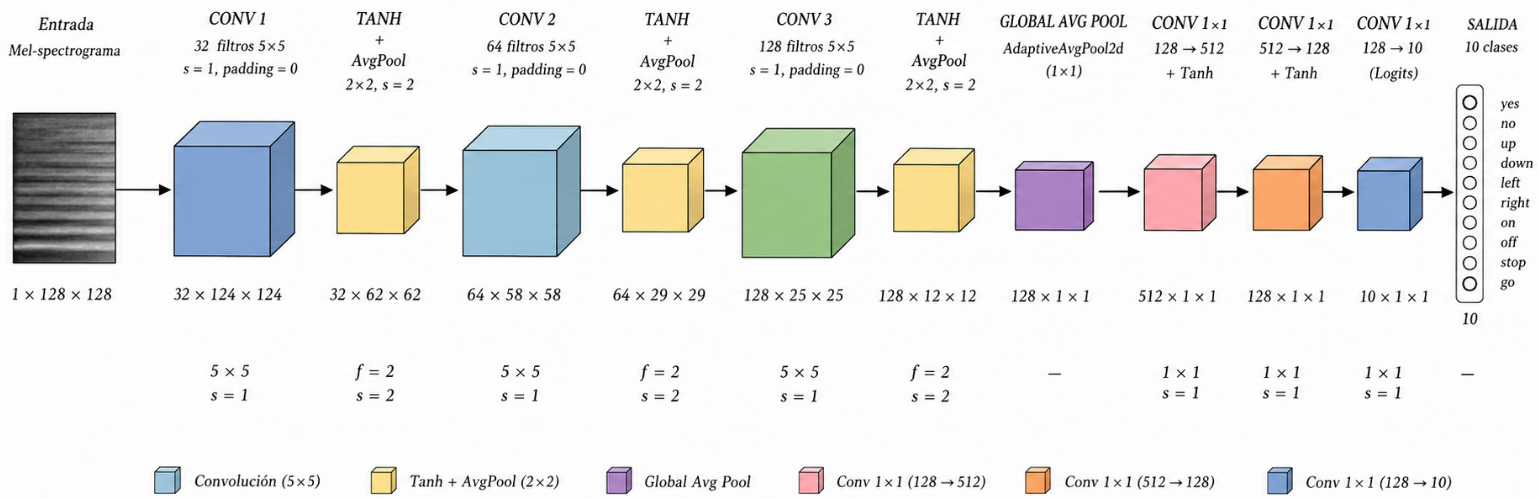
\includegraphics[width=\linewidth]{images/Modelo_LeNet5_adaptado.png}}
\caption{Diagrama visual de la arquitectura del Modelo A.}
\label{fig:model_a}
\end{figure}

\subsubsection{Función de Pérdida, Optimizador y Entrenamiento}
Se utilizó \textit{Cross-Entropy Loss} como función de pérdida, la cual es ideal para clasificación multiclase. El optimizador seleccionado fue \texttt{Adam} con una tasa de aprendizaje de $1 \times 10^{-3}$ y \textit{weight decay} de $1 \times 10^{-4}$ para mitigar el sobreajuste. Además, se empleó un \textit{scheduler} (\texttt{ReduceLROnPlateau}) que reduce la tasa de aprendizaje a la mitad si la precisión de validación no mejora en 3 épocas. Las rutinas de entrenamiento se ejecutaron usando precisión mixta nativa (\texttt{torch.amp}).


\section{Análisis y comparación de resultados}

\subsection{Modelo A: Datos crudos}

El modelo A (sin aumento de datos y empleando la arquitectura 100\% convolucional) logró resultados sumamente robustos en la fase de prueba (\textit{testing}), alcanzando un \textbf{Accuracy global de 89.84\%} y un \textbf{Loss de 0.2838}. El F1-Score macro fue de 0.8973, lo que demuestra un equilibrio excelente entre las clases y refleja que la arquitectura generaliza muy bien sin memorizar los datos. El detalle de las métricas por clase se expone en la Tabla \ref{tab:metricas_a}.

\begin{table}[htbp]
\caption{Reporte de Clasificación - Modelo A (datos crudos)}
\label{tab:metricas_a}
\centering
\begin{tabular}{lcccc}
\toprule
\textbf{Comando} & \textbf{Precision} & \textbf{Recall} & \textbf{F1-Score} & \textbf{Support} \\
\midrule
yes   & 0.94 & 0.93 & 0.93 & 637 \\
no    & 0.90 & 0.89 & 0.89 & 608 \\
up    & 0.85 & 0.86 & 0.85 & 551 \\
down  & 0.88 & 0.86 & 0.87 & 520 \\
left  & 0.91 & 0.92 & 0.91 & 600 \\
right & 0.93 & 0.94 & 0.93 & 575 \\
on    & 0.93 & 0.89 & 0.91 & 572 \\
off   & 0.84 & 0.85 & 0.84 & 549 \\
stop  & 0.94 & 0.92 & 0.93 & 579 \\
go    & 0.88 & 0.90 & 0.89 & 524 \\
\midrule
\textbf{Accuracy} & \multicolumn{3}{c}{\textbf{0.90}} & \textbf{5715} \\
\textbf{Macro Avg}& \textbf{0.90} & \textbf{0.90} & \textbf{0.90} & \textbf{5715} \\
\bottomrule
\end{tabular}
\end{table}

A pesar de no utilizar aumento de datos, el análisis de las curvas de aprendizaje (Figura \ref{fig:curvas_a}) evidencia un comportamiento muy saludable para un modelo con \textit{Global Average Pooling}:

\begin{figure}[htbp]
\centerline{
\includegraphics[width=\linewidth]{images/Graficas_Modelo_A_raw.png}}
\caption{Curvas de entrenamiento: Loss, Accuracy y F1-Score.}
\label{fig:curvas_a}
\end{figure}

Al evaluar las métricas de las épocas finales, se observa lo siguiente:
\begin{itemize}
    \item \textbf{Train Acc:} Alcanzó un $\sim 90.3\%$. No llegó al 100\%, evitando la memorización del \textit{dataset}.
    \item \textbf{Val Acc:} Terminó acompañando de cerca al \textit{Train Acc} rondando un $\sim 88.9\%$, lo que denota excelente capacidad de generalización.
    \item \textbf{Train Loss:} Descendió y se estabilizó gradualmente hasta $0.277$.
    \item \textbf{Val Loss:} Se mantuvo alineado con la pérdida de entrenamiento terminando alrededor de $0.318$, sin mostrar aquellos clásicos y drásticos aumentos repentinos comunes en etapas avanzadas de memorización.
\end{itemize}

El modelo logra mitigar casi en su totalidad el agresivo fenómeno de \textbf{Overfitting (sobreajuste)}. La reducción drástica de parámetros al reemplazar las capas densas por convoluciones de $1 \times 1$ forzó a la red a sintetizar los patrones espectrales de manera más global en todo el espectrograma (gracias al \textit{pooling} promedio). Aún así, la implementación posterior de técnicas de \textit{Data Augmentation} sigue estando en los planes recomendados para robustecer el modelo contra la variación de ambientes acústicos externos y llevar la precisión más allá del 90\%.

\begin{figure}[htbp]
\centerline{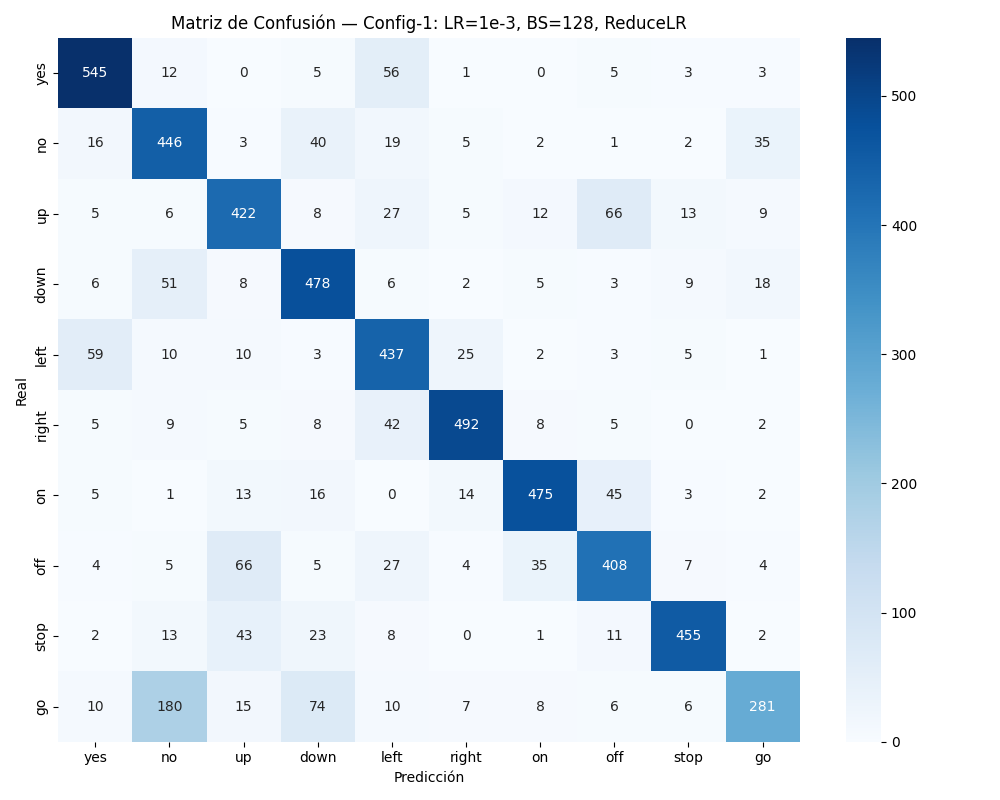
\includegraphics[width=\linewidth]{images/Matriz_Confusion_Modelo_A_raw.png}}
\caption{Matriz de confusión del Modelo A (datos crudos) sobre los datos de prueba.}
\label{fig:matriz_a}
\end{figure}

En la matriz de confusión (Figura \ref{fig:matriz_a}), se puede observar que a pesar de que el rediseño redujo ampliamente el sobrentrenamiento e hizo al modelo más uniforme para dispositivos móviles, aún hay pares de comandos (falsos positivos/negativos) donde ocurren confusiones debido a similitudes fonéticas. El \textit{data augmentation} será esencial para ayudar al Global Average Pooling a discernir mejor algunas de estas ambigüedades acústicas en etapas futuras.

\section{Referencias}
\begin{thebibliography}{00}

\end{thebibliography}

\end{document}